\chapter{Introduction and Related Work}
\section{Introduction}
%\cite{Kato1998,Prasad2013,Lindegaard2003,Ridley2003,Perez2002,JUNKINS1991}
Two-thirds of the earth is covered by the ocean and the underwater robots can help us to explore and perform various tasks in this hazardous and uneasily attainable environment. The autonomous underwater vehicles (AUVs) have various application areas. For scientific purpose, they can be used for seafloor mapping or geological sampling. In the environmental area, people utilize them to inspect the underwater structures like pipelines, dams, etc. or to monitor the pollution. Besides, underwater robots also bring convenience to the ocean survey and undersea structures' construction and maintenance~\cite{Yuh2000}. 

A good manoeuvring performance of underwater robots requires an appropriate robot structure adapting to the specific mission. This is a tough and time-consuming task involving many iterations of design and testing, even though for skilled expert. A simple underwater robot prototype includes CPU, the inertial navigation system, the sensory and communication system, and the power supply system (batteries). All of them are enclosed in a protecting hull. Besides, thruster and control fins are the main actuators. Their properties, numbers and locations will influence the robot's working performance heavily. Hence, a good designer should be able to find a suitable configuration of these components.

Traditionally, after the robot was built by the designer, the users will analyse the dynamics based on the current robot structure and actuator configuration. Then they will plan the trajectory and design the controller based on this dynamic model and the task requirements. 

In this work, we separate the hull design and the actuator placement optimization. Designing the hull should satisfy the conventional specifications: buoyancy neutral, maximal surge velocity, maximal working time and low construction cost and a minimal volume to contain the inertial measurement unit, CPU and communication system. In terms of the actuator design we start from an innovative designing direction. That is, a set of requirements for kinematics and dynamics is directly derived from a set of trajectories the vehicle should perform. A suitable trajectory representation should be chosen and key requirements should be identified. In the design phase, an automated co-design of the optimal kinematics and dynamics of the robot together with the synthesis of a stable controller for tracking is aimed for. 

In Chapter 2, we propose a modular modeling method for the underwater robot prototype. Each component can be modeled as sample geometric shape determined by several geometric variables and then we can parametrize the robot dynamics with these variables. 

From deep-sea exploration to underwater rescue, underwater vehicles require efficient path planning algorithms. An relative simple but representative trajectory is expected for designing the robot. So we use the trim trajectory since robot's motion is stable along them. Partial kinematic states ($\phi$, $\theta$), the dynamic states (linear and angular velocities) that influence the robot dynamics and therefore the hydrodynamic coefficients depending on velocities stay constant along the trim trajectory. A set of desired trim trajectories give us firstly information about the desired position for the robots. By adopting the Frenet-Serret frame, the desired orientation and the desired velocity along the trajectory will be derived in further. With the full information about the system states, we are able to formulate the error dynamics. These will be introduced in Chapter 3. 

For analysis and controller design of nonlinear systems the typical approach is to linearize the nonlinear system. In this work we adopt a trajectory-based linearization way for the error dynamics usd in~\cite{Silvestre2002} for the following reasons. Firstly, for a specific trim trajectory segment the linearized error dynamics is unique. Hence, we can implement a number of analysing approaches for linear systems for the error dynamics. Secondly, tracking a desired trajectory is a concern for practical manoeuvring tasks. The error dynamic formulation along trim trajectories will be illustrated in Chapter 4. Moreover, task-specific trajectories for underwater robots can be planned as a combination of a set of trim trajectories, which means that we also have a set of linearized MIMO error dynamics. Thus, we design a switched LQR controller based on these linear systems. This will also be discussed in the same chapter.    

The main contribution of this work is to find an optimal geometric configuration of the robot constituent parts. Based on the parametrized underwater vehicle model built in Chapter 2, we are able to identify the relationship between the geometric decision variables and each term in the dynamic model (the mass matrix, the Coriolis matrix, the damping matrix and the restoring matrix). After that, we propose two optimization algorithms which find a locally optimal hull size and a local optimum for actuator placement, respectively.

In Chapter 6, we utilize the geometry from the optimization results and calculate the corresponding optimal dynamics. Regular underwater robots are normally equipped with actuators symmetrically in pairs. These new built robots are visualized to provide us a more intuitive impression about the irregular robots. The irregularity      is caused by the randomly generated initial geometric decision variables and the nonlinear optimization algorithm that is only able to find a local minimum depending on the initial values. The controllability of the current designed robot system is verified by means of checking the tracking performance along a set of trim trajectories. 

Underwater dynamics are nonlinear, highly coupled, MIMO systems with six degrees of freedom (DOFs). When we change
the geometric parameters of hull and actuators or the number of actuators, the geometric center, the center of buoyancy, the inertia matrix, the Coriolis matrix and the hydrodynamic damping will also change consequently. In addition, the modeling of thrusters and control fins is not accurate enough to indicate their real physical characteristics. To make the optimization solvable, we make a list of assumptions. These inaccuracies can be rectified and the optimization performance can be enhanced for future works. These limitations and the possible improvements will be discussed in the last chapter. 

The complete underwater robot designing and verification processes proposed in this thesis are concluded in Figures~\ref{FIG:DesignPhase} and~\ref{FIG:VerificationPhase}. 
\begin{figure}
\centering
\includegraphics[width=0.95\textwidth]{DesignPhase.eps}
\caption{Underwater robot geometric design procedure}	
\label{FIG:DesignPhase}
\end{figure}
\begin{figure}
\centering
\includegraphics[width=0.7\textwidth]{VerificationPhase.eps}
\caption{Verification of geometric design}	
\label{FIG:VerificationPhase}
\end{figure}
\section{Related Work}
Our work draws from a number of ideas and methods from underwater robot modelling, error dynamics and controller design and computational robot design.
\subsection{Underwater Robot Modular Dynamic Modeling}
The chapter 7 of~\cite{F2011} introduces 1 DOF heading autopilot model, 3DOF manoeuvring and dynamic positioning (DP) models, 4 DOF manoeuvring and 6 DOF coupled system for advanced 6DOF manoeuvring model. Especially for underwater robots with actuation in all DOFs, a nonlinear, strongly coupled, MIMO dynamic 6DOF model is required for the model-based controller and observer design. The detailed derivation can be found in the appendix \ref{Appendix:DM} summarized from~\cite{F2011,F1994,FF1995,AG2014}.

Our goal is to design algorithms finding an optimal configuration for AUVs. It requires the robots to have a flexible modularized structure so that we can reconfigure the robot prototype easily.  In~\cite{Vasilescu2005}, a novel modular  underwater robot which can self-reconfigure by stacking and unstacking its component modules is designed. A modular dynamic modeling is desired for this flexible robot structure. With help of this method, the dynamic equation can be parametrized with geometric variables (location, size etc.) and especially the hydrodynamic coefficients can be estimated from them. The modular modeling methods are discussed in~\cite{Chen2007} and~\cite{Sia1999}.
\subsection{Controller Design and Path Planning}
Due to the requirement of full-DOF control, underwater robot control is a very challenge task. Diverse control methods can be implemented for the robot, e.g., adaptive control (\cite{JYuh1990,Svein1991}), sliding model control (\cite{JSoltine1985,Narimani2006}), feedback linearization (\cite{Wadoo2003}), backstepping (\cite{Jian2015,Wadoo2003}).

In~\cite{Makdah2016}, the 6 degrees of freedom (6DOF) dynamics and kinematics model of the underwater robots is linearized about the given desired trajectory. A linear time variant (LTV) state space model for underwater robots is obtained. And then a linear quadratic controller is designed according the linear models and applied to the nonlinear robot dynamics to track the desired trajectory. Our idea is very similar to this, we also want to linearize the nonlinear model along the trajectory. However, since we should utilize the linear models for the following optimization algorithm, a relative small number of linearized models is expected for the given trajectory. By special nonlinear transformation~\cite{RNC705} along trim trajectory, the error dynamics between the real robot states and the trajectory-determined states can be uniquely linearized, which satisfies our trajectory design aim. The trim trajectory is widely used for unmanned aerial vehicles (UAVs) because of its simplicity for controling and analysing. Its benefits and practical usages can be found in~\cite{Beji2005,Bottasso2008,Sebbane2015}.
   
\subsection{Computational Design}
The basic idea of this work was inspired from~\cite{Du2016}. In this paper, Du et al. proposed  an  interactive  procedure to computationally design, optimize, and fabricate multicopters. The multicopter can be constructed from  a  collection  of  components including propellers, motors, and carbon fiber rods. They proposed an algorithm optimizing shape and controller parameters of the current design to ensure the multicopter's proper operation. Other merics including payload, battery usage, size, and cost are integrated into the optimization algorithm.

Generally speaking, both underwater robot and multicopter has the 6DOF dynamics. In spite of this, the underwater robots usually have full 6DOF actuation and thus contain a number of equilibrium points, while the multicopter stays at the equilibrium when the total resultant thrust equal to the gravity and the total result moment is equal to zero. In addition, beside the thrusters the underwater robots have also fins as control surfaces and their hydrodynamic characteristics are nonlinear and of high-order. The underwater robots possess a more complicated structure, making the geometric optimization a challenging task.

There are still a lot other works concerning the computational design of robots. In~\cite{Schulz2014}, a data-driven method for designing 3D models that can be fabricated was proposed. Schulz et al. propose the end-to-end system for design of robots with ground locomotion~\cite{Schulz2017}. The biggest advantage of the computational design is that it allows people of all skill level to design and fabricate robots.   

\subsection{Geometric Optimization}
\cite{JOUNG201244} present a methodology to optimize the AUV profile in order to reduce the total resistance with Computational Fluid Dynamics (CFD). The majority of works in terms of actuator optimization discusses the control allocation problem, e.g \cite{Fossen2008,Johansen2004,Johansen2005}.

In~\cite{XU20151044}, Xu et al. propose a novel local optimization of thruster configuration based on a synthesized  positioning  capability  criterion.

In our work, we optimize not only the hull but also the actuator configuration and our actuator includes thrusters and control fins. The control location problem normally formulated as optimization problems whose objective is to produce the specified generalized forces to minimize the control effort (power consumption), the position of thrusters is already fixed after the robot design is finished. In this case, the decision variables are normally the azimuth angle of the thrusters and the forces generated by them. Our optimizations are performed during the design phase. Hence, our decision variables contain not only the thrust forces, more importantly, an optimal thruster location should be found. Similarly, the deflection angle and the fin location should be optimized at the same time. 

\section{Contributions}
To summarize, our main contribution in this work include:
\begin{itemize}
\item Deriving the design requirements for robot kinematics and dynamics from a set of trim trajectories.
%\item Identifying important geometric variables determining the underwater robot dynamics. Define  are identified and the underwater robot dynamics is parametrized by these parameters; 
\item Approximating each constituent module of the underwater robot as a simple shape determined by several geometric decision variables and building the robot dynamics parametrized with them.
\item Identifying the couplings among all geometric decision variables.
\item Formulating an optimization problem that can optimize the size of the robot hull enclosure according to different design specifications.
\item Formulating an optimization problem that can jointly optimize positions and orientations, spin directions and control parameters satisfying the trajectory-based design requirements. 
\item Linearizing and transforming the nonlinear underwater robot dynamic system into a linear switched system, designing the switched Linear Quadratic Regulator (LQR) for the system.
\item Finding the state cost matrices and the input cost matrices for the switched  
LQR based on the stability.
\item Providing an efficient numerical approach to solve the actuator placement optimization by using the multi-stage iterative optimization method.
%\item  Providing an efficient numerical method to solve the underwater robot optimization problem and show its efficacy by optimizing different types of non-standard underwater robots
\end{itemize}







